%----------------------------------------------------------------------------------------
%	PACKAGES AND THEMES
%----------------------------------------------------------------------------------------
\documentclass[aspectratio=169,xcolor=dvipsnames]{beamer}
\usetheme{SimpleDarkBlue}

\usepackage{hyperref}
\usepackage{graphicx} % Allows including images
\usepackage{booktabs} % Allows the use of \toprule, \midrule and \bottomrule in tables
\usepackage{caption}
\usepackage{subcaption}

\usepackage[magyar]{babel}


%----------------------------------------------------------------------------------------
%	TITLE PAGE
%----------------------------------------------------------------------------------------

\title[short title]{Az MRC-100 műhold SZTE-s diákmoduljának áramköri kihívásai és megoldásai} % The short title appears at the bottom of every slide, the full title is only on the title page
\subtitle{}

\author[Antal Levente] {Antal Levente}

\institute[NTU] % Your institution as it will appear on the bottom of every slide, may be shorthand to save space
{
    SZTE Móra Ferenc Szakkollégium \\
    Szegedi Tudományegyetem , BSc Villamosmérnöki
     % Your institution for the title page
    \vskip 3pt
}
\date{\today} % Date, can be changed to a custom date


%----------------------------------------------------------------------------------------
%	PRESENTATION SLIDES
%----------------------------------------------------------------------------------------

\begin{document}

\begin{frame}
    % Print the title page as the first slide
    \titlepage
\end{frame}

\begin{frame}{Áttekintés}
    
    \tableofcontents
\end{frame}

%------------------------------------------------
\section{Bevezetés}
\section{Geometriai és technológiai megkötések}
\section{Alkatrészek választásának szempontjai}
\section{Áramköri megvalósítások}
\section{Befejezés}
%------------------------------------------------

\begin{frame}{Bevezetés}
	\begin{columns}[c]
	\column{.2\textwidth}

	\begin{itemize}
        \item Indíttatás
	\item PocketQube
	\end{itemize}

	\column{.4\textwidth}
	\begin{figure}[h]
	\centering
		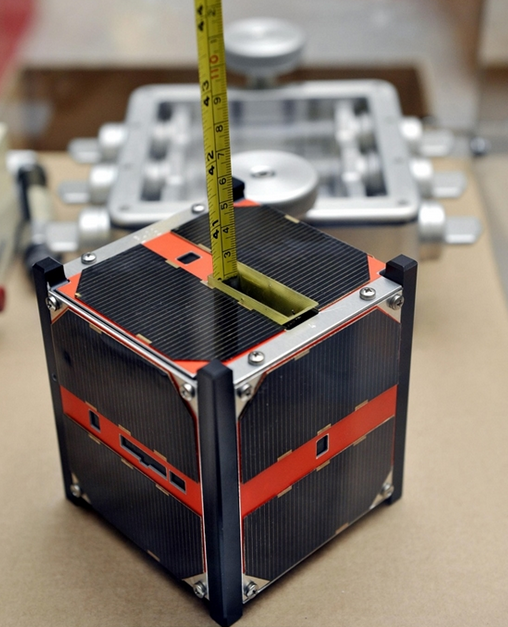
\includegraphics[width=0.4\linewidth]{masat.png}
		\caption{MASAT-1}

	\end{figure}
	\column{.4\textwidth}
	\begin{figure}[h]
		\centering
		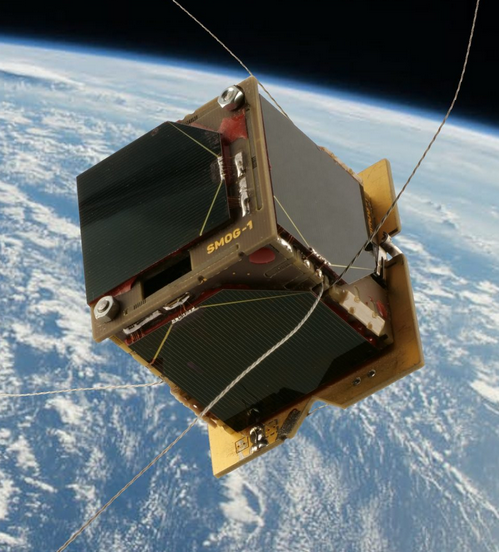
\includegraphics[width=0.45\linewidth]{smog1.png}
		\caption{SMOG-1}
	\end{figure}

	\end{columns}

\end{frame}

%-----------------------------------------------

\begin{frame}{Geometriai és technológiai megkötések}


	\begin{columns}[c]
	\column{.6\textwidth}
		\begin{itemize}
		\item Konvenciók
		\begin{itemize}
			\item Méret : 30 x 30 x 3 mm
			\item Tömeg : max 50 g
			\item 0,8 - 1,5 mm vastag FR-4-es áramköri hordozó
		\end{itemize}
		\item Forrasztás
			\begin{itemize}
				\item Forrasztás gátló lakk használata \alert{TILOS}
				\item Ólommentes anyaggal való forrasztás \alert{TILOS}
				\item Folyasztószer használata \alert{TILOS}
			\end{itemize}
		\item Alkatrészek pozícionálása
	\end{itemize}


	\column{.5\textwidth}
		\begin{figure}[h]
		\centering
		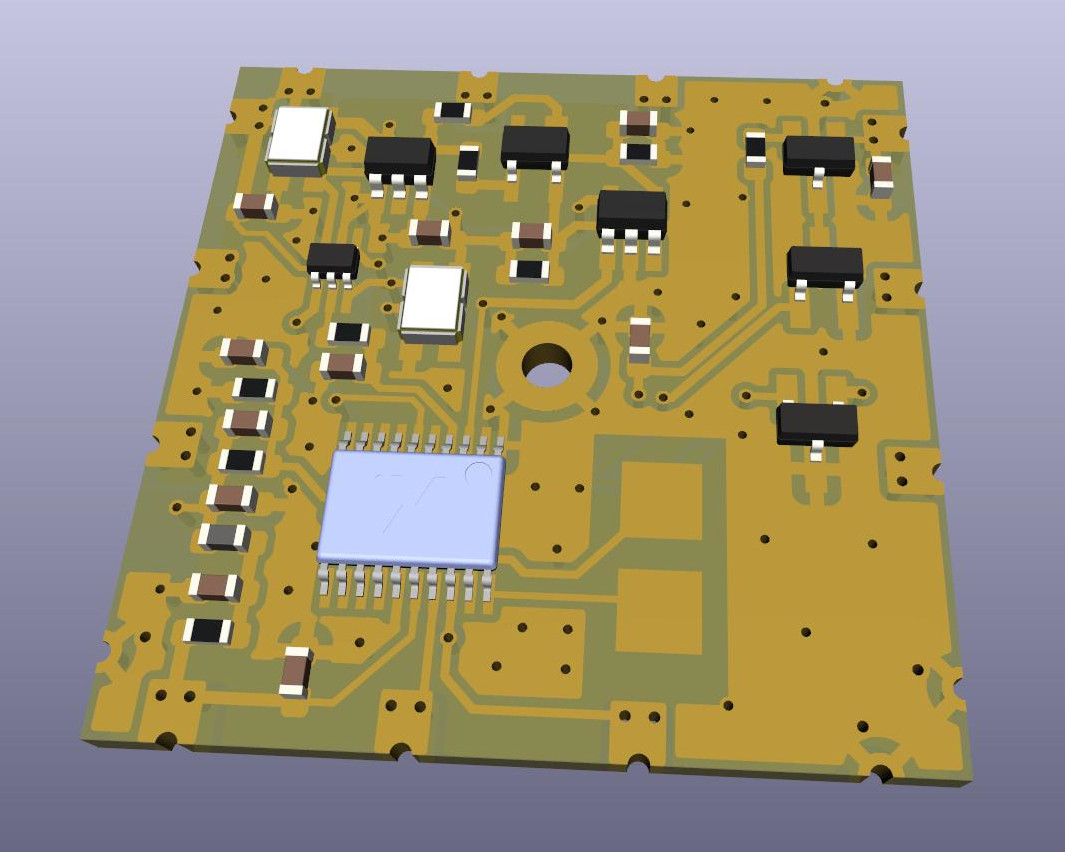
\includegraphics[width=0.5\textwidth]{3d_render}
		\caption{3D render image}
		\end{figure}
		

	\end{columns}

  
\end{frame}


\begin{frame}{Hitelesített tömegmérés}
	\begin{figure}[h]
		\centering
	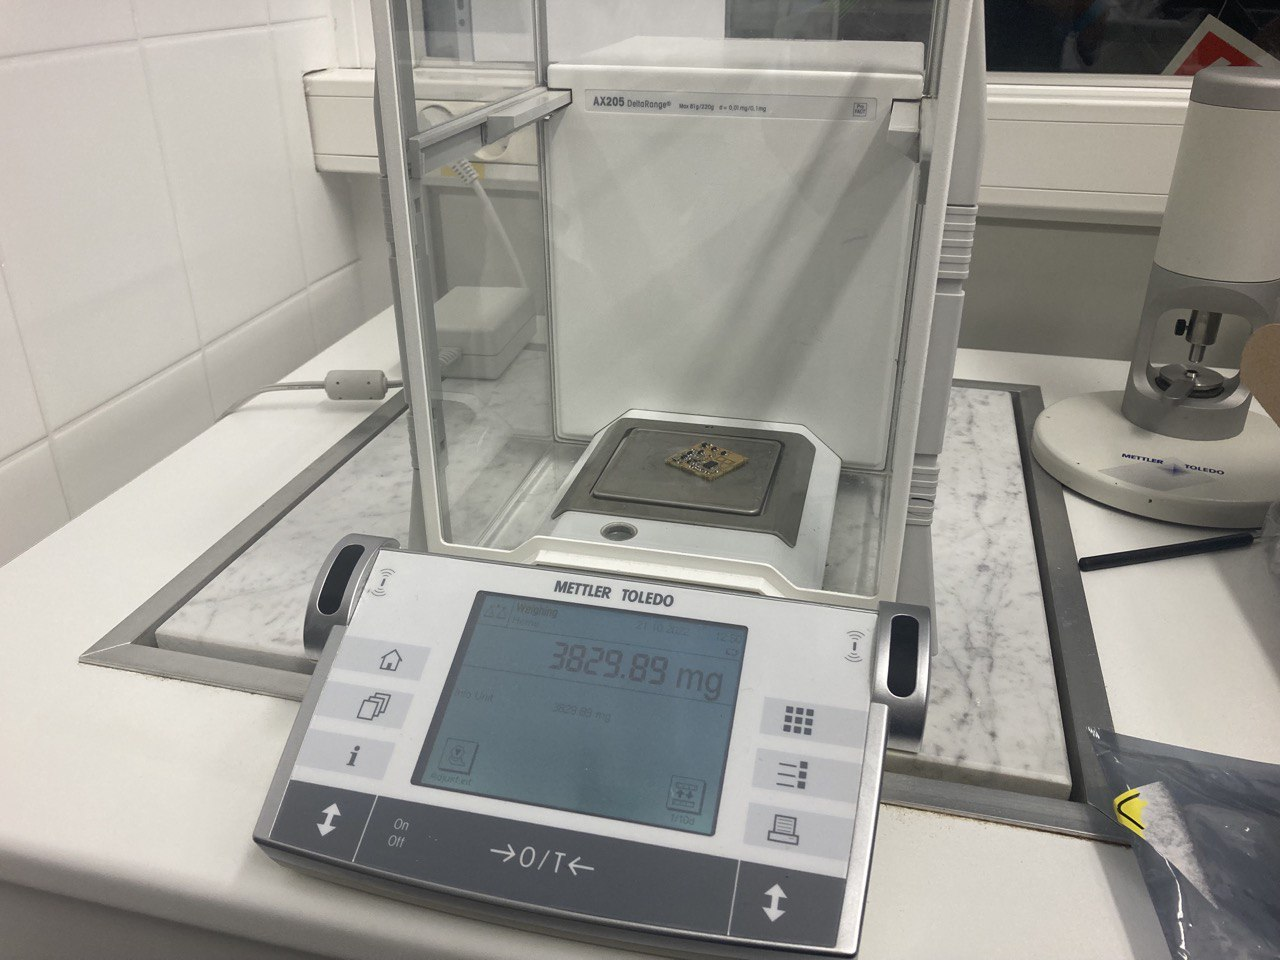
\includegraphics[width=0.6\textwidth]{tomeg}
		\caption{A modul hitelesített tömege}
	\end{figure}

\end{frame}





%------------------------------------------------

\begin{frame}{Alkatrészek választása}
    \begin{columns}[c] 

        \column{.4\textwidth} % Left column and width
       
        \begin{itemize}
            \item{- 40 - 85 \textdegree C hőmérséklet tartomány}
            \item X5R és X7R technológia
	    \item Redundancia fontossága
        

        \end{itemize}

        \column{.6\textwidth} 
       
		\begin{figure}[h]
		\centering
			
			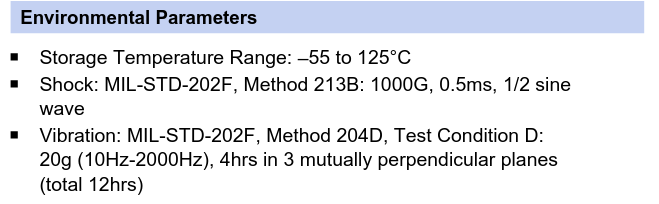
\includegraphics[width=0.7\textwidth]{oscillator}

		\caption{Az oszcillátor tűrése} 
		\end{figure}

    \end{columns}


\end{frame}

\begin{frame}{Áramköri megvalósítások}

	\begin{columns}[c]
	\column{.45\textwidth}
	\begin{enumerate}
	\item Redundáns oszcillátor áramkör
	\item ADC zaj mérése kiegyenlített osztóval
	\item Hall szenzoros mérés
	\item Hőmérséklet mérése
	\end{enumerate}
	\column{.5\textwidth}
		\begin{figure}[h]
		\centering
			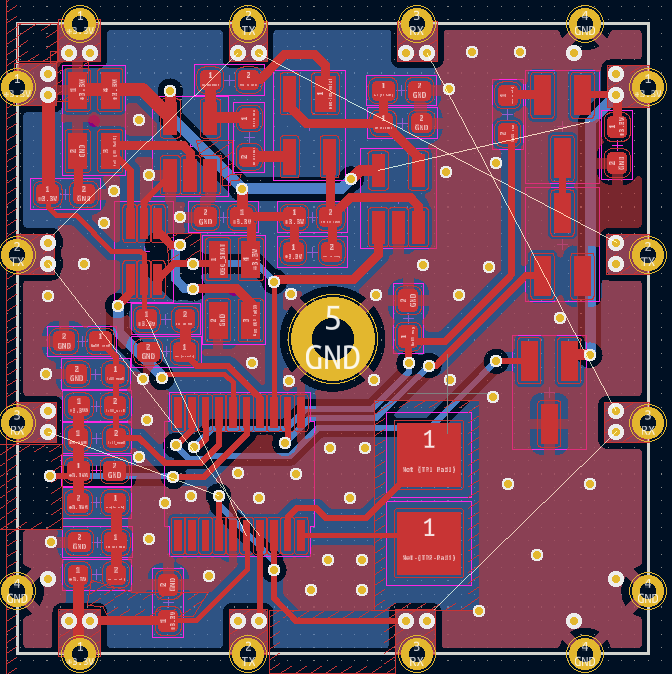
\includegraphics[width=0.6\textwidth]{nyak}
			
		\caption{Nyomtatott huzalozású lemez}
		\end{figure}
	\end{columns}


\end{frame}


\begin{frame}{Redundáns oszcillátor áramkör}

	\begin{figure}[h]
		\centering
		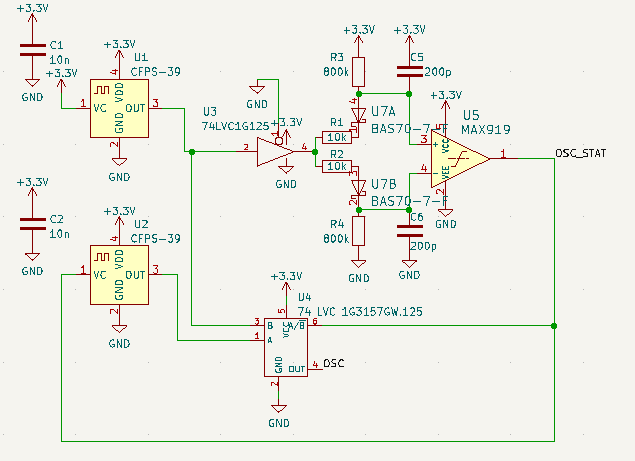
\includegraphics[width=0.6\textwidth]{redundant}
		\caption{Redundáns oszcillátor áramkör}
	\end{figure}

	\end{frame}


\begin{frame}{Kísérletekhez használt áramkörök}

	\begin{figure}[h]
		\centering
		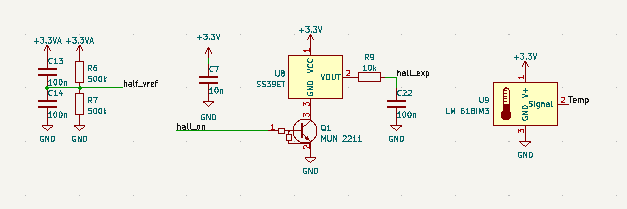
\includegraphics[width=0.7\textwidth]{kiserletek}
		\caption{Kísérletekhez használt áramkörök, balról : ADC , HALL , TMP}
		\end{figure}

	\end{frame}

\begin{frame}{Chiphiány}
	\begin{columns}[c]
	\column{.5\textwidth}

			\begin{figure}[h]
				\centering
			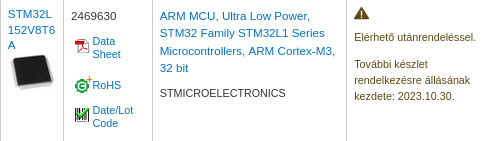
\includegraphics[width=0.7\textwidth]{chip1}
				\caption{Chiphiány}
			\end{figure}

	\column{.5\textwidth}
		\begin{figure}[h]
		\centering
			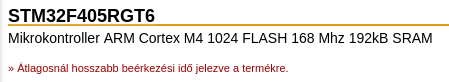
\includegraphics[width=0.7\textwidth]{chip2}
			
		\caption{Chiphiány}
		\end{figure}
	\end{columns}

\end{frame}

\begin{frame}{Szponzoraink}

\includegraphics[width=0.2\linewidth]{fdh}

\includegraphics[width=0.2\linewidth]{ret}
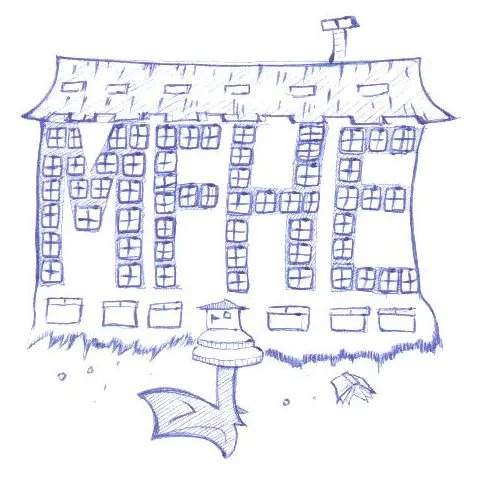
\includegraphics[width=0.2\linewidth]{mfhe}

\includegraphics[width=0.15\linewidth]{eurocircuits}

\includegraphics[width=0.2\linewidth]{csiha}
\end{frame}

\begin{frame}{Felhasznált nyílt kódú szoftverek}
	\LaTeX
	
\includegraphics[width=0.1\linewidth]{manjaro}
	
\includegraphics[width=0.1\linewidth]{linux}
	
\includegraphics[width=0.1\linewidth]{kicad}
	
\includegraphics[width=0.1\linewidth]{kdevelop}
	
\includegraphics[width=0.1\linewidth]{gcc}
	
\includegraphics[width=0.1\linewidth]{gdb}
	
\includegraphics[width=0.1\linewidth]{make}
	
\includegraphics[width=0.1\linewidth]{vim}
	
\includegraphics[width=0.1\linewidth]{llvm}
	
\includegraphics[width=0.1\linewidth]{bash}
	
\includegraphics[width=0.1\linewidth]{git}
	
\includegraphics[width=0.1\linewidth]{kde}
	
\includegraphics[width=0.1\linewidth]{gnome}
\end{frame}


\begin{frame}
    \Huge{\centerline{Köszönöm a figyelmet!}}
\end{frame}

\end{document}
